\documentclass[final]{beamer}
\usepackage{eulervm,verbatim}          
\usepackage[scaled]{helvet}
\usepackage[most]{tcolorbox}
\setbeamercolor{frametitle}{fg=black,bg=white} % Colors of the block titles
\setbeamertemplate{caption}{\raggedright\insertcaption\par}
\setbeamertemplate{caption}{\raggedright\insertcaption\par}
\definecolor{darkcerulean}{rgb}{0.03, 0.27, 0.49}
\newcommand{\citesmall}[1]{[{\color{darkcerulean}\begin{small} \textbf{#1} \end{small}}]}
\setbeamertemplate{footline}[frame number]
\DeclareMathOperator*{\argmin}{arg\,min}
\usepackage{graphicx}  % Required for including images
\usepackage{bbm}
\usepackage{booktabs} % Top and bottom rules for tables
\definecolor{burgundy}{rgb}{0.5, 0.0, 0.13}
\newcommand{\highlight}[1]{{\color{burgundy} \textbf{#1}}}
\usepackage{hyperref}
\hypersetup{
    colorlinks=true,
    linkcolor=blue,
    filecolor=magenta,      
    urlcolor=magenta,
    pdftitle={CSE6740-Lecture 14},
    pdfauthor={Nisha Chandramoorthy},
    pdflang={en-US}
}



%----------------------------------------------------------------------------------------
%	TITLE SECTION 
%----------------------------------------------------------------------------------------
\title{\begin{huge}{Lecture 17: Midterm 1 and problem-solving}\end{huge}} % Poster title


\author{Nisha Chandramoorthy} % Author(s)


%----------------------------------------------------------------------------------------

\begin{document}

\frame{\titlepage}

%----------------------------------------------------------------------------------------
%	OBJECTIVES
%----------------------------------------------------------------------------------------
\begin{frame}{Notes}
\begin{itemize}
\item Best of two will be considered
\pause
\item Proposal: 1 page, due 2nd Nov
\pause
\item Last time: VCDim of FCNN, VC generalization bounds, then implementation  
\pause
\item Today: Midterm 1 and problem-solving
\pause
\item After this: CNNs, VAEs, feature extraction/Dimension reduction
\end{itemize}
\end{frame}
\begin{frame}{Asking questions}
\begin{figure}
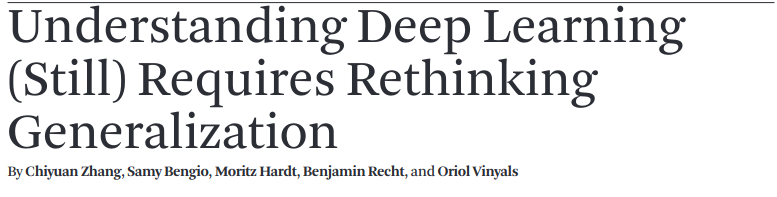
\includegraphics[width=\textwidth]{paperTitle.png}
\end{figure}
\begin{itemize}
\item Training data consists of random labels.
\end{itemize}
\pause
	\begin{figure}
	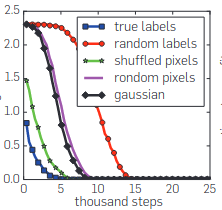
\includegraphics[width=0.4\textwidth]{trainingError.png}
	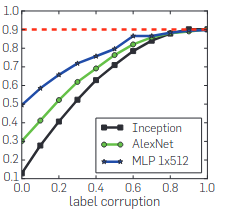
\includegraphics[width=0.4\textwidth]{testError.png}
	\end{figure}
\end{frame}
\begin{frame}{Does our understanding of generalization hold?}
\begin{figure}
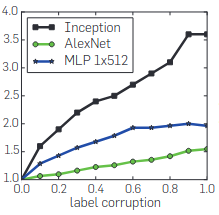
\includegraphics[width=0.6\textwidth]{trainingTime.png}
\end{figure}

\begin{itemize}
	\item Hand-wavy: test error is higher when we expect complexity to be higher.

\end{itemize}

\end{frame}
\begin{frame}{How to improve generalization?}
	\begin{figure}
		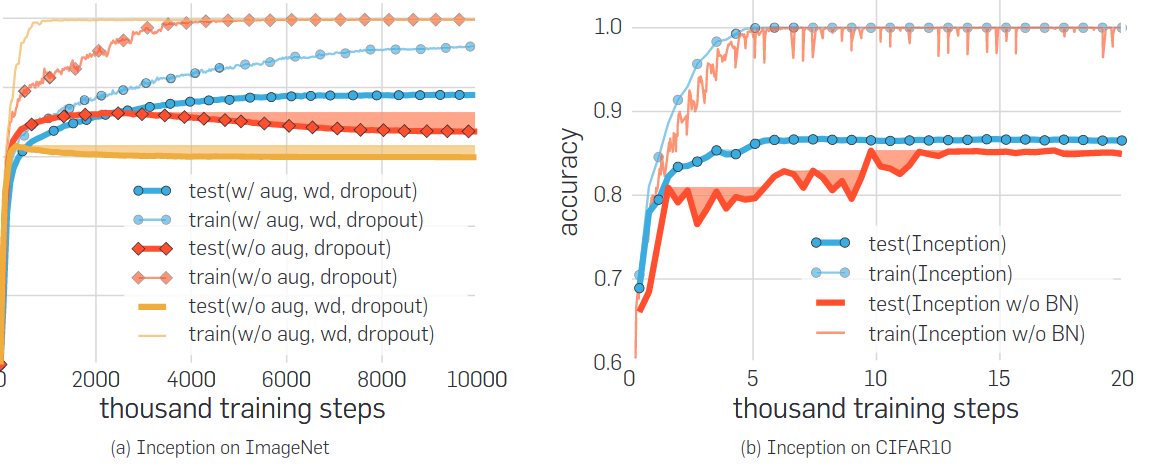
\includegraphics[width=\textwidth]{effectOfRegularization.png}
	\end{figure}
	\begin{itemize}
		\item Early stopping (implicit regularization)
		\pause
		\item Batch normalization: normalize the inputs to each layer for each mini-batch, i.e., make the inputs have zero mean and unit variance.
		\pause
		\item Dropout: randomly set some activations to zero. 
	\end{itemize}

\end{frame}
\begin{frame}{What is the conclusion?}
\begin{itemize}
	\item Bias-complexity tradeoff
	\pause
	\item Need to get new ideas/insights into generalization
	\pause
	\item The role of the data distribution...
	\pause
	\item Bubeck Sellke 2021:
	\begin{figure}
	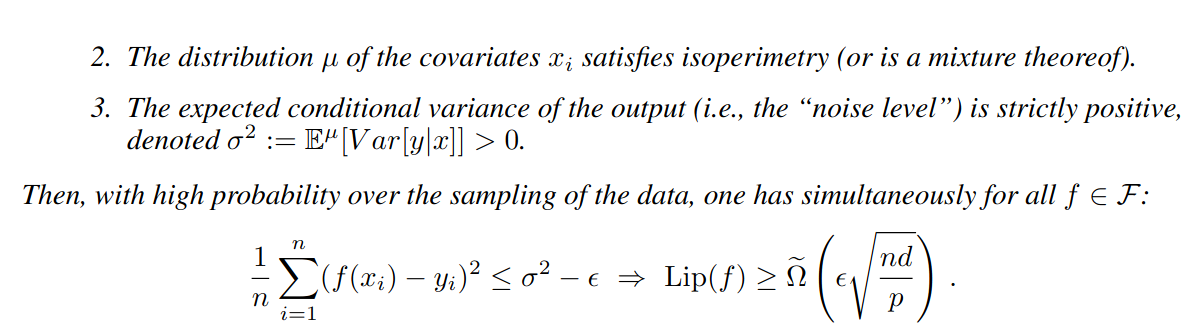
\includegraphics[width=\textwidth]{bubeckSellke.png}
	\end{figure}

\end{itemize}
\end{frame}
\begin{frame}{What are the assumptions?}
	\begin{itemize}
		\item Isoperimetry: if for an $l$-Lipschitz function $h:\mathbb{R}^d\to\mathbb{R},$ $\mathbb{P}[|h(X) - E h|\geq t]\leq 2 e^{(-dt^2)/(2 cl^2)},$ then, the distribution of $X$ is $c$-isoperimetric. 
		\item for learning smooth functions (${\rm Lip}(f)\leq l$), the number of parameters is $\Omega(nd\epsilon^2/l)$
		\pause
	\item For imagenet, Bubeck and Sellke estimate needing ${\cal O}(10^{10}-10^{11})$ parameters.
	\end{itemize}

\end{frame}
\begin{frame}{Thinking from first principles}
	\begin{itemize}
		\item Kernel ridge regression: ``Simply applying
a Gaussian kernel on pixels and using no regularization
			achieves 46\% test error." [Zhang et al 2021]
		\pause
		\item ``By preprocessing with a random
convolutional neural net with 32,000 random filters, this
test error drops to 17\% error'' [Zhang et al 2021]
		\pause
		\item $\ell^2$ regularization leads to better generalization. Why?



	\end{itemize}
\end{frame}
\begin{frame}{Regularization and generalization}
	\begin{itemize}
	\item  ``the $\ell^2$-norm of the minimum
norm solution with no preprocessing is approximately
220. With wavelet preprocessing, the norm jumps to 390.
Yet the test error drops by a factor of 2'' [Zhang et al 2021]
	\pause
	\item ``So while this minimum-norm intuition may provide some guidance to new
algorithm design, it is only a very small piece of the generalization story''
	\pause
	\item Rademacher complexity of linear class (on features) lower. 
	
	\end{itemize}
\end{frame}
\begin{frame}{Developing computational thinking}
	\begin{itemize}
		\item Theoretical and computational problems are always intertwined
		\pause
	\item Spending time (struggling) with problems productively
		\pause
		\item Crisis, reflection on concepts that lead to resolution
		\pause
		\item Implementing algorithms improves understanding
		\pause
		\item Reading papers, books, but working on your own
		\pause
		
		\item Question-first approach may be more efficient
		\pause
		\item Pattern-matching is non-trivial
		\pause
		\item Repetition helps!
	\end{itemize}
\end{frame}
\begin{frame}{Having the right attitude toward grad school courses and research}
	\begin{itemize}
		\item Computational science: intersection of math, data science, computer science, and domain science
		\pause
		\item Developing computational thinking takes time
		\pause
		\item Difficulties compounded by various intersections!
		\pause
		\item No need to panic or despair or feel inadequate!
		\pause
		\item Flourishing? ``Mathematics for human flourishing'' - Francis Su

	\end{itemize}
\end{frame}

\end{document}
